\section{Atomic orbitals: radial distributions and slices}
\label{sec:atomic-orbitals}
\index{Atomic orbitals}
\index{Orbitals!atomic|see{Atomic orbitals}}
\index{Argon}
\checkedwith{9.5.3-dev}{9aa88a4ce}
\eccexample{Examples > General Chemistry > Atoms}
\helppage{density-profile}

\helppage{density-map}

The orbitals of an atom are usually drawn as boundary surfaces, a sphere for s and two lobes for p, and such a drawing hides most of what the principal quantum number does. This chapter looks at the occupied orbitals of argon in two other ways, as a curve of probability against the distance from the nucleus and as a contour map on a flat slice through the nucleus. Both views come from the same stored calculation and show the nodes, the inner maxima of 2s, 3s and 3p, and the three shells of argon.
\index{Shells}\index{Nodes}\index{Inner maxima}

\subsection{Background}
\index{Radial distribution}
\index{Radial distribution function|see{Radial distribution}}
\index{Orbitals!radial distribution|see{Radial distribution}}
\index{Probability of finding an electron|see{Radial distribution}}
An orbital $\psi(r,\theta,\phi)$ of an atom gives, through $|\psi|^2$, the probability per unit volume of finding the electron at a point. The question asked of an atom is more often how far from the nucleus the electron is, in any direction, and the answer is the radial distribution function
\begin{equation}
	P(r) = r^2 \oint |\psi(r,\theta,\phi)|^2 \, d\Omega ,
	\label{eq:rdf}
\end{equation}
the probability per unit distance of finding the electron in a thin spherical shell of radius $r$. For a normalised orbital $\int_0^\infty P(r)\,dr = 1$. For a hydrogen-like atom the orbital separates into a radial part $R_{nl}(r)$ and a spherical harmonic, and Eq.~\eqref{eq:rdf} reduces to $P(r) = r^2 R_{nl}^2(r)$. The factor $r^2$, which is the area of the sphere apart from $4\pi$, makes $P(r)$ zero at the nucleus even for an s orbital, whose density $|\psi|^2$ is largest there.

The radial part has $n-l-1$ nodes, spheres on which $\psi$ is zero and changes sign, and the orbital has $l$ angular nodes besides, planes or cones through the nucleus, so $n-1$ nodes in all.
\index{Nodes!radial}\index{Nodes!angular}\index{Nodal plane}
Between consecutive radial nodes $P(r)$ has a maximum, which gives $n-l$ maxima: one for 1s, 2p and 3d, two for 2s and 3p, three for 3s. The outermost maximum is the largest and sets the size of the orbital; the others are the inner maxima. The position of the largest maximum is the most probable radius,
\index{Most probable radius}\index{Inner maxima}
which for a hydrogen-like orbital with $l = n-1$, one without a radial node, is
\begin{equation}
	r_\mathrm{mp} = \frac{n^2 a_0}{Z},
	\label{eq:rmp}
\end{equation}
with $a_0 = \SI{0.529}{\angstrom}$ the Bohr radius and $Z$ the nuclear charge; for 1s it is $a_0/Z$.

The inner maxima are the origin of penetration.
\index{Penetration}\index{Shielding}
A 2s electron has a small maximum inside the 1s shell, close to the nucleus, where the two 1s electrons screen little of the nuclear charge, and a 2p electron has no such maximum. The 2s electron therefore feels a larger effective nuclear charge on average and lies lower in energy, which is why 2s fills before 2p and, in the next period, 3s before 3p (Section~\ref{sec:periodic-trends}). Slater's screening rules put these trends into numbers \cite{slater1930}.
\index{Effective nuclear charge}

In a many-electron atom the orbitals are no longer hydrogen-like, but the counting of nodes and maxima survives. The total electron density of argon, summed over the occupied orbitals and weighted by $r^2$, has one hump for each filled shell: 1s close to the nucleus, then 2s and 2p together, then 3s and 3p.

\subsection{What ECCE shows}
\index{Density Profile}\index{Density Map}
\index{Properties list!Density Profile}\index{Properties list!Density Map}
The Atoms topic of the General Chemistry example set holds ECCE-QM calculations of 21 atoms, H to Ar, Ca, Cr and Cu.
\index{ECCE-QM}\index{Codes!ECCE-QM}\index{Example calculations!General Chemistry}
The argon calculation uses B3LYP \cite{becke1993} with the aug-cc-pVTZ basis set \cite{woon1993}, is closed shell, and gives a total energy of $-527.490442$~hartree. Its nine occupied orbitals are 1s ($-115.118$~hartree), 2s ($-11.142$), three 2p ($-8.693$), 3s ($-0.968$) and three 3p ($-0.426$).
\index{B3LYP}\index{Basis sets!aug-cc-pVTZ}\index{Orbital energies!argon}

Two panels in the Orbitals group of the \menu{Properties} list work from the orbital coefficients and the basis set stored with the calculation. The \menu{Density Profile} plots a quantity against one length; for a single atom it opens on \menu{Around an atom}, where \menu{Radial distribution} is Eq.~\eqref{eq:rdf} evaluated for each chosen orbital and \menu{Spherical average of $\psi^2$} is the same average without the $r^2$.
\index{Density Profile!Around an atom}\index{Density Profile!Radial distribution}\index{Density Profile!Spherical average of psi2@Spherical average of $\psi^2$}
The \menu{r axis} can be \menu{Linear}, \menu{$\sqrt{r}$} or \menu{log r}; the square root spreads out the region near the nucleus, where the inner shells are, while the tick marks stay in $r$ itself.
\index{Density Profile!r axis}\index{Square-root axis}
On a $\sqrt{r}$ axis the area under a curve is no longer the number of electrons, and the panel says so beneath the plot, where the note also gives the most probable distance of each curve.
\index{Most probable radius!in the Density Profile}

The \menu{Density Map} draws one orbital, or the density, as contour lines on a flat slice. A single atom opens on \menu{This view (parallel to the screen)}, a plane through the nucleus. With \menu{Show: One orbital} the positive values are drawn as solid blue lines and the negative values as dashed vermilion lines, so that a node lies where the two colours meet; the levels start at $\pm 0.02$ and double.
\index{Density Map!One orbital}\index{Density Map!This view (parallel to the screen)}\index{Contour map}\index{Orbitals!sign|see{Phase}}\index{Phase}
The \menu{MO} box chooses the orbital, and the mouse wheel zooms the map about the pointer.

\subsection{Procedure}
\index{Opening example calculations}
\index{File menu!Open Example Calculations}
\index{Organizer!Open Example Calculations}
\index{Viewer}
\begin{enumerate}
	\item In the Organizer, choose \menu{File > Open Example Calculations}, pick \menu{General Chemistry} and click \menu{OK}. The calculations go into the project \menu{Examples}, sorted into topics.
	\item In the topic \menu{Atoms}, select the calculation \menu{Ar} and click \menu{Viewer}.
	\item In the \menu{Properties} list, click \menu{Density Profile}. The panel opens on \menu{Around an atom} with \menu{Centre} \menu{Ar1}.
	\index{Density Profile!Centre}
	\item Choose \menu{Radial distribution} and \menu{Selected orbitals}, and in the list of orbitals tick 1s, 2s and 3s and untick the others.
	\index{Density Profile!Selected orbitals}
	\item Set \menu{r axis} to \menu{$\sqrt{r}$}.
	\item To zoom, turn the mouse wheel over the plot or drag a rectangle; double-click to return to the whole plot, or click \ctrl{Show all}.
	\index{Density Profile!Show all}\index{Zooming a plot}
	\item Tick 2p, 3s and 3p instead.
	\item In the \menu{Properties} list, click \menu{Density Map} and choose \menu{Show: One orbital}.
	\item Step through the occupied orbitals 1 to 9 with the arrows of the \menu{MO} box, drawn as \ctrl{$-$} and \ctrl{+} buttons. The caption above the map names the orbital, its energy and its occupation.
	\index{Density Map!MO box}\index{Stepping through orbitals}
	\item Turn the mouse wheel over the nucleus to zoom in; double-click the map, or click \ctrl{Whole plane}, to see all of it again.
	\index{Density Map!Whole plane}\index{Zooming a map}
\end{enumerate}

\subsection{Results}
\index{Shells!of argon}
Figure~\ref{fig:ao-rdf1} shows the radial distributions of 1s, 2s and 3s on the $\sqrt{r}$ axis. 1s has a single maximum, at a most probable distance of \SI{0.0299}{\angstrom} according to the note under the plot. Equation~\eqref{eq:rmp} with $Z = 18$ gives $a_0/18 = \SI{0.0294}{\angstrom}$, and the slightly larger value is the screening of one 1s electron by the other, corresponding to an effective nuclear charge of about 17.7. 2s has one node and two maxima, the smaller at about the distance of the 1s maximum, and 3s has two nodes and three maxima, the inner two at about the distances of the 1s and 2s maxima. The number of nodes rises by one with each step in $n$. The most probable distances of 2s and 3s are \XXX[ read from the note under the plot].
\index{Effective nuclear charge}

\begin{figure}[htb]
	\centering
	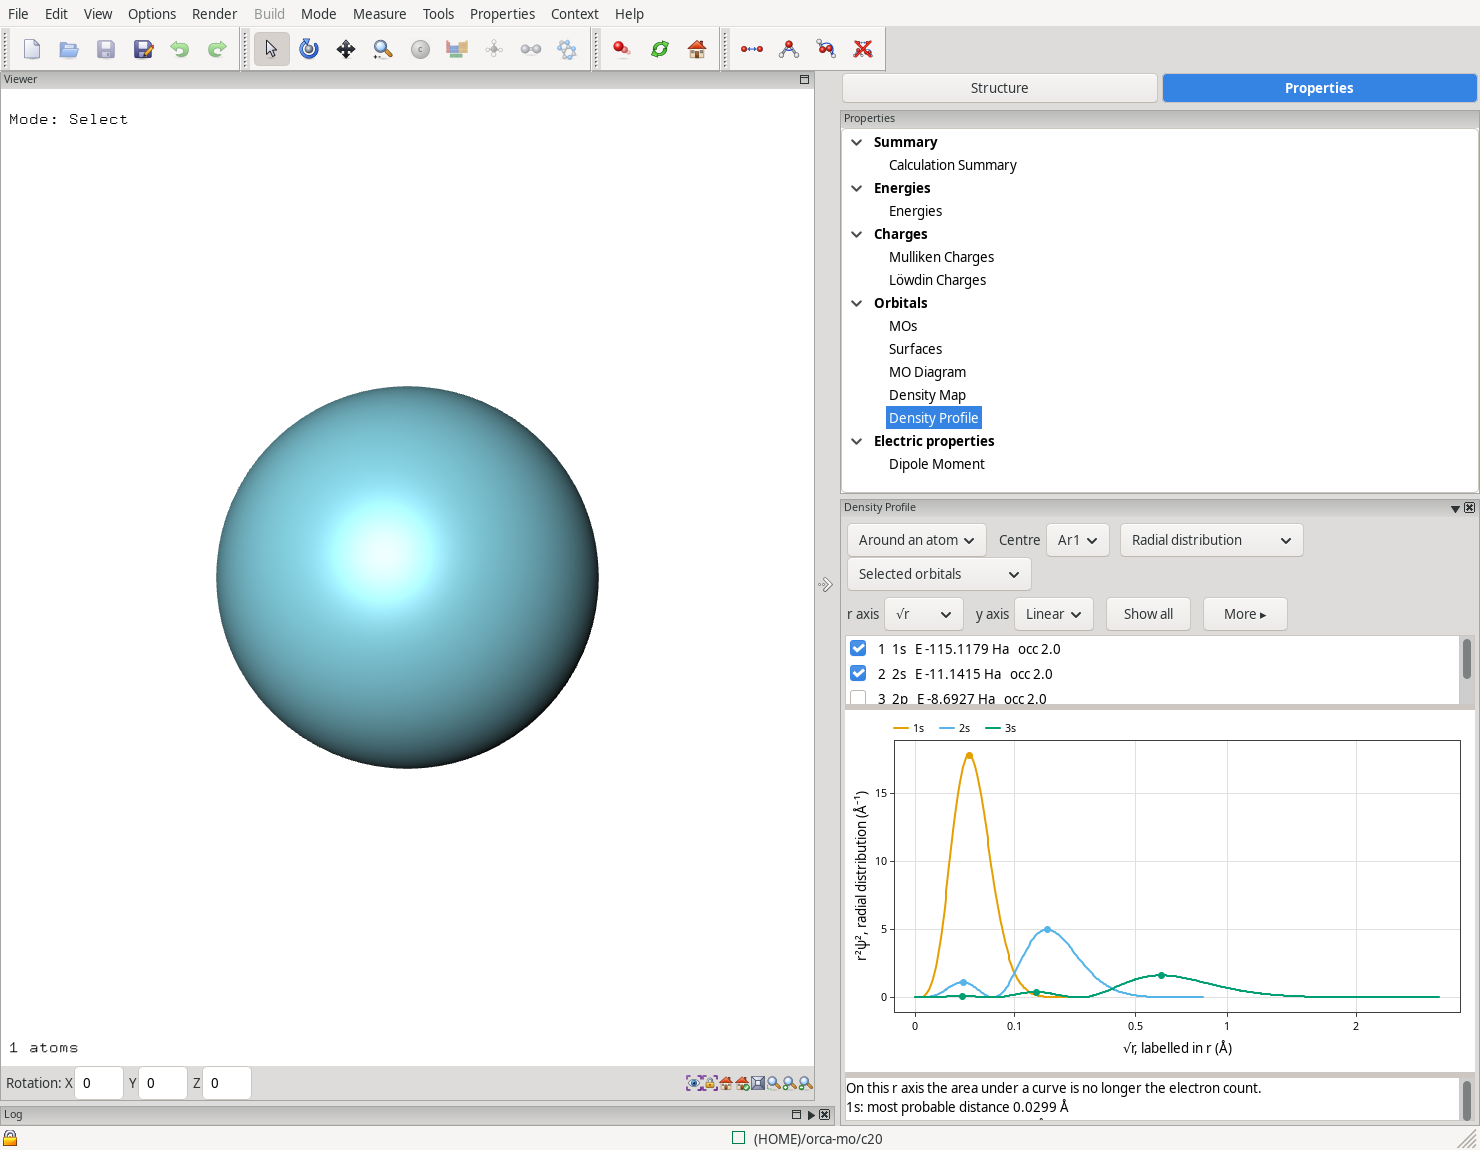
\includegraphics[width=\linewidth]{atomic-orbitals/rdf1.ecce-unknown.png}
	\caption{Argon in the Viewer, with the \menu{Density Profile} on \menu{Around an atom}, \menu{Radial distribution}, \menu{Selected orbitals} 1s, 2s and 3s and a $\sqrt{r}$ axis. \XXX[ screenshot shows a \menu{More} button where the help names \menu{Options}; regenerate from the Atoms example.]}
	\label{fig:ao-rdf1}
\end{figure}

With 2p, 3s and 3p ticked (Fig.~\ref{fig:ao-rdf2}), 2p has a single maximum and no node, and 3p has one node and two maxima. The main maxima of 3s and 3p lie at about the same distance, that of 3p slightly further out, which is what makes them one shell. Their inner maxima differ, since 3p has one, near the 2p maximum, while 3s has a second one closer still to the nucleus, at about the 1s maximum. A 3s electron therefore penetrates further than a 3p electron, and the orbital energies follow, $-0.968$~hartree for 3s against $-0.426$~hartree for 3p.
\index{Penetration!3s and 3p}

\begin{figure}[htb]
	\centering
	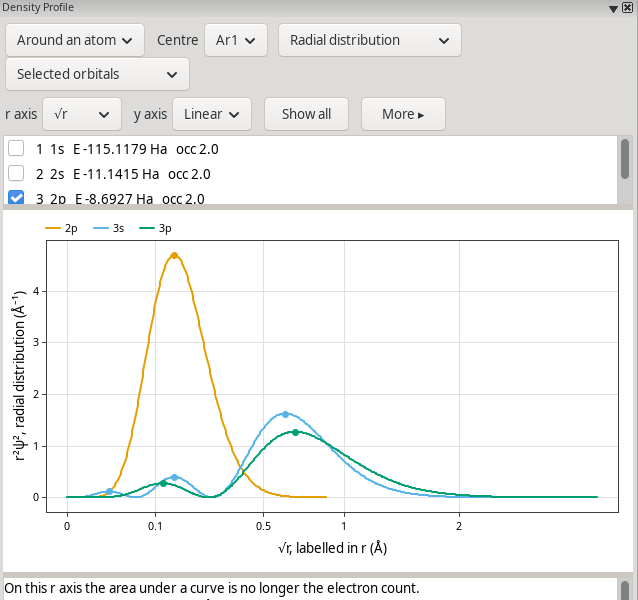
\includegraphics[width=0.75\linewidth]{atomic-orbitals/rdf2.ecce-unknown.png}
	\caption{The \menu{Density Profile} of argon with 2p, 3s and 3p ticked.}
	\label{fig:ao-rdf2}
\end{figure}

The total density of argon, with its three shells, is not among the figures yet. \XXX[ screenshot: Ar, \menu{Density Profile}, \menu{Around an atom}, \menu{Radial distribution}, \menu{Total only}, \menu{r axis} $\sqrt{r}$, showing the three humps of the total for 1s, 2s+2p and 3s+3p.]

In the \menu{Density Map} (Fig.~\ref{fig:ao-map}) orbital 6 is 3s. The circles of the contour map are the spherical nodes of the radial distribution seen edge-on. Going out from the nucleus the sign changes twice, which gives a small disc about the nucleus, a ring of opposite sign around it and the large outer part, with the sign of the disc. The disc and the ring are the two inner maxima of Fig.~\ref{fig:ao-rdf1}, and the zoomed map (Fig.~\ref{fig:ao-mapzoom}) shows how close to the nucleus they lie. The sign of 1s does not change at all, and that of 2s changes once.

\begin{figure}[htb]
	\centering
	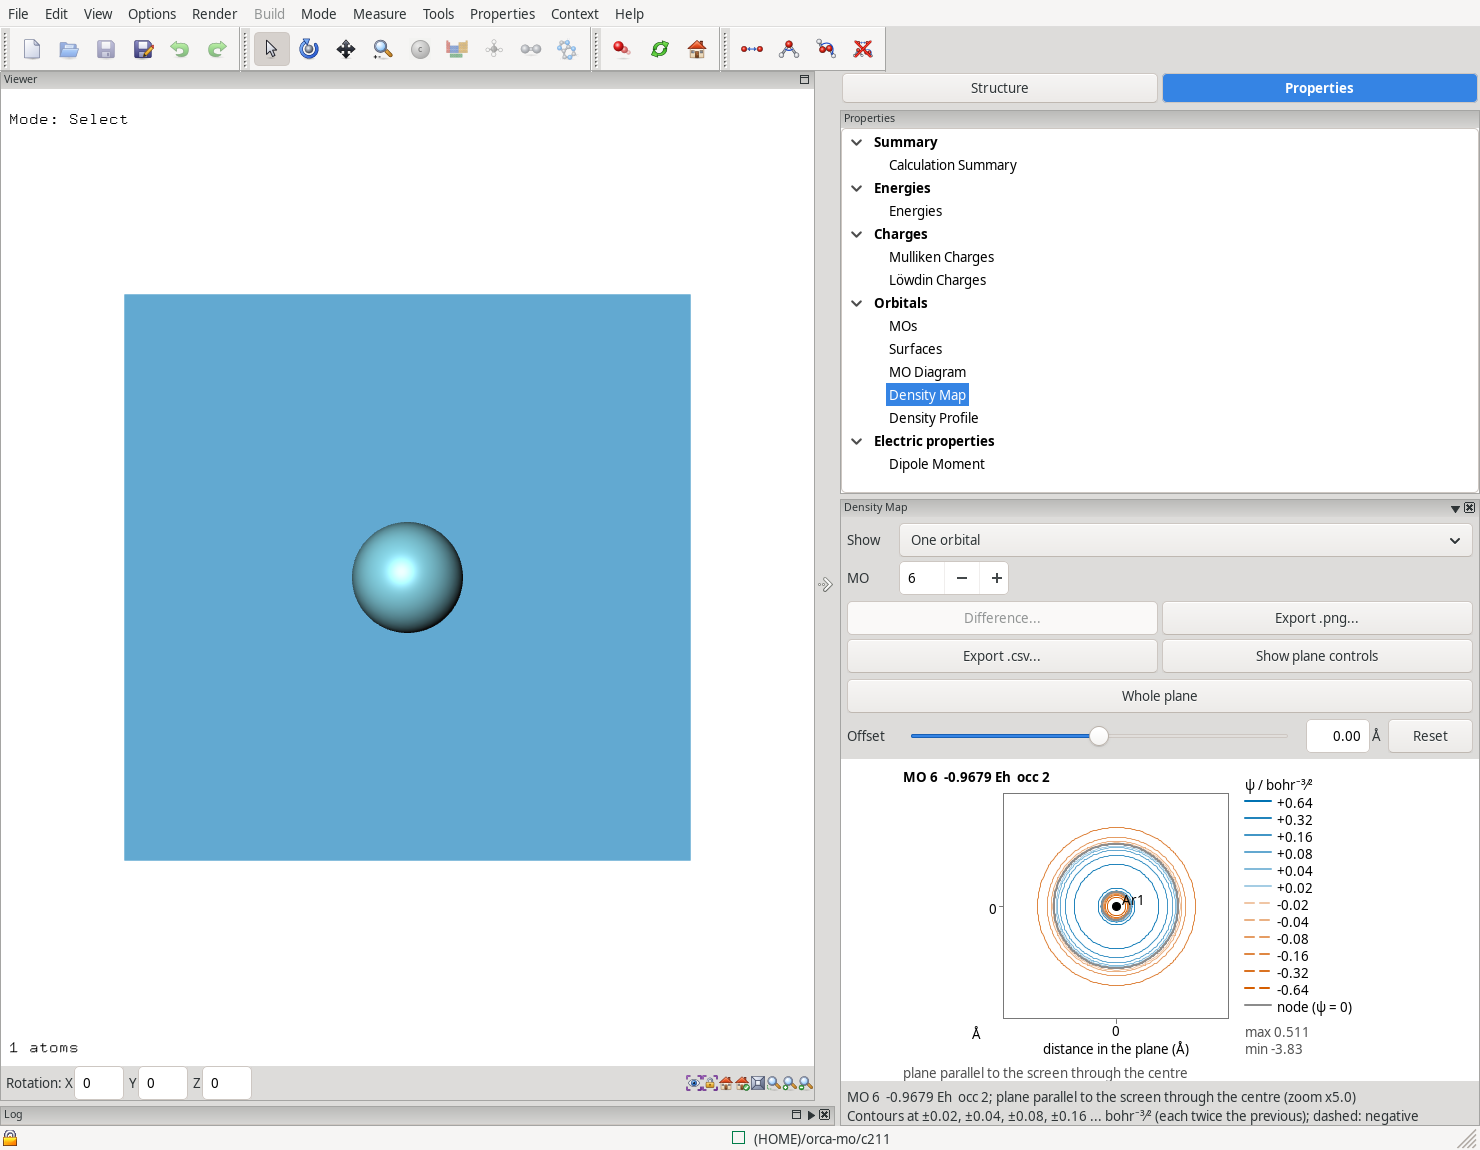
\includegraphics[width=\linewidth]{atomic-orbitals/map1.ecce-unknown.png}
	\caption{Argon with the \menu{Density Map} on \menu{One orbital}, MO 6 (3s, $-0.9679$~hartree), on the plane parallel to the screen through the nucleus; the slice is drawn in the 3-D view as a translucent square. \XXX[ screenshot shows a \menu{Show plane controls} button where the help names \menu{Options}; regenerate.]}
	\label{fig:ao-map}
\end{figure}

\begin{figure}[htb]
	\centering
	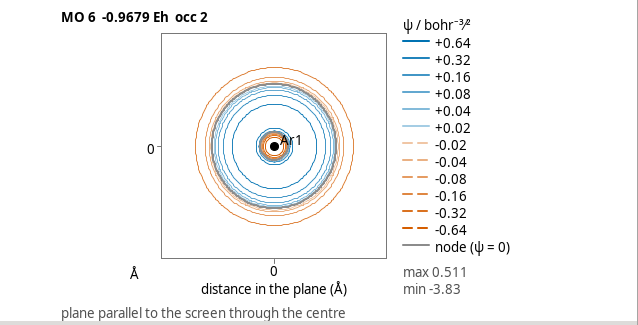
\includegraphics[width=0.75\linewidth]{atomic-orbitals/map1zoom.ecce-unknown.png}
	\caption{The map of Fig.~\ref{fig:ao-map}, zoomed in on the nucleus.}
	\label{fig:ao-mapzoom}
\end{figure}

The 2p and 3p orbitals each have a nodal plane through the nucleus, and the slice cuts the three members of each set differently: a member lying in the slice shows two lobes of opposite sign on either side of the nodal line, while one pointing out of the slice can look almost empty. \XXX[ screenshot: Ar, \menu{Density Map}, \menu{One orbital}, the member of MO 3--5 (2p) that lies in the plane, zoomed in, showing the nodal plane as a line.]
\index{Nodal plane}

\subsection{History}
Schrödinger solved the wave equation of the hydrogen atom in 1926, which gave the radial functions and their nodes \cite{schrodinger1926}, and Slater set out his rules for the screening of the nuclear charge in 1930 \cite{slater1930}.
\index{History!Schrödinger}\index{History!Slater}
